\documentclass[11pt]{article}

% --- packages (all standard; compiles on stock TeX Live / Overleaf) ---------
\usepackage[margin=1in]{geometry}
\usepackage[T1]{fontenc}
\usepackage{lmodern}
\usepackage{amsmath,amssymb,amsthm}
\usepackage{booktabs}
\usepackage{graphicx}
\usepackage{xcolor}
\usepackage{caption}
\usepackage[hidelinks]{hyperref}
\usepackage{microtype}

\graphicspath{{figures/}}

% --- theorem environments ---------------------------------------------------
\theoremstyle{plain}
\newtheorem{theorem}{Theorem}
\newtheorem{proposition}{Proposition}
\newtheorem{lemma}{Lemma}
\newtheorem{corollary}{Corollary}
\newtheorem{conjecture}{Conjecture}
\theoremstyle{definition}
\newtheorem{definition}{Definition}
\theoremstyle{remark}
\newtheorem{remark}{Remark}

% --- shorthand --------------------------------------------------------------
\newcommand{\xstar}{x^{\!*}}
\newcommand{\pg}{p_{\text{g}}}
\newcommand{\reps}{r}
\newcommand{\Rzero}{R_{0}}
\newcommand{\norm}[1]{\left\lVert #1 \right\rVert}
\DeclareMathOperator*{\argmax}{arg\,max}
\DeclareMathOperator*{\argmin}{arg\,min}

\title{\bfseries Contagious Context:\\[2pt]
Self-Reproducing and Transmissible Token Strings\\
in a Markov Cache}
\author{Dan Shumow\thanks{Write-up of the analysis in the open-source project
\texttt{trust-is-the-attack-surface} (branch \texttt{context-contagion}), built on the toy
model \texttt{markov-models-aux-context-caching}. Every figure and number is reproduced by
the \texttt{demo\_contagion*.py} scripts in that repository.}}
\date{June 2026}

\begin{document}
\maketitle

\begin{abstract}
A companion analysis~\cite{shumow2026trust} showed, on a toy global-plus-cache Markov
model, that in-context exploitability tracks \emph{trust}---the weight a model places on its
context---and that in \emph{generation} a single self-reinforcing injected count undergoes a
\emph{condensation} transition, locking in once trust is high enough. This paper asks what a
single locked token generalizes to: can a whole \emph{string} be made to reproduce itself,
and can it \emph{spread} between contexts? We treat the cache as the host of a self-replicating
payload and make three contributions, all exact on the toy. (i) \textbf{Payload.} We
characterize \emph{quines}---strings an empty cache regenerates when run generatively. Exact
reproduction obeys a window-distinctness theorem (an order-$k$ quine of period $p$ has $p$
distinct $k$-windows and hence no proper sub-cycle), per-step fidelity follows a closed form
$\rho+(1-\rho)\pg$, and the cost to plant a contagious string splits white-box vs.\ black-box
with a gap $a\,T\,\pg$ that vanishes for stealthy payloads. For \emph{approximate} quines,
period \emph{divisibility} gates a sub-cycle collapse: composite-period strings fall onto
their largest proper divisor, prime-period strings are harmonic-protected. (ii)
\textbf{Delivery.} Infecting a cache already warmed on a legitimate document factors as
$\text{entry}\times\text{lock-in}$; the cheapest \emph{bridge} context balances visit
frequency against single-count leverage subject to a frequency ceiling, a black-box attacker
recovers the optimum from observation alone, and jointly optimizing entry and lock-in saves
$3$--$4\times$ over over-provisioning lock-in (the minimum sits at the condensation knee).
(iii) \textbf{Transmission.} When a host that \emph{reads} an infected output re-injects the
copies it saw, one passage is a map $k_{\text{in}}\!\to\!k_{\text{out}}$ with a basic
reproduction number $\Rzero\!\approx\!T/(p\,k_{\text{thresh}})$: short strings are epidemic,
and there is a \emph{critical length} above which the worm dies out after the index host.
Finally, re-running all three parts under the toy's \emph{induction} (longest-match)
surrogate---its model of a transformer copy mechanism---makes self-reproducing strings several
times cheaper to plant, erases the order and length penalties, and lets far longer worms
sustain: contagion is most acute exactly where induction dominates.
\end{abstract}

% ===========================================================================
\section{Introduction}\label{sec:intro}
% ===========================================================================
A language model carries two memories: the frozen weights and the context window. Poisoning
the context window---through retrieved documents, tool output, or prior turns---is a live
threat~\cite{greshake2023,cohen2024}, and a companion paper~\cite{shumow2026trust} studied it
on a deliberately minimal surrogate: a global (parametric) Markov model linearly combined
with an online Markov \emph{cache} standing in for in-context learning. The headline there was
that \emph{exploitability tracks trust, not usefulness}, and a striking corollary appeared in
generation. Because sampling a symbol increments its own count, the generative process is a
nonlinear P\'olya urn~\cite{pemantle2007}, and a single self-reinforcing injected count
exhibits a \emph{condensation} transition: shrugged off below a trust threshold, locked in
above it.

That last result is about \emph{one} token getting stuck. This paper takes it as a starting
gun. If a single self-reinforcing element can capture generation, then (a) a structured
\emph{string} of tokens might be engineered to regenerate itself---a context-window analogue
of \emph{echolalia}, the compulsive repetition of what was just heard---and (b) such a string,
once emitted, might be \emph{read} by another context and reproduce there, i.e.\ spread. The
end state is a self-replicating prompt, the toy-model cousin of the LLM ``worms'' demonstrated
against real RAG pipelines~\cite{cohen2024}. We are after the quantitative skeleton of that
phenomenon: what strings reproduce, how cheaply they can be planted in an occupied cache, and
when reproduction within a host becomes an epidemic across hosts.

The reason to ask these questions of the toy is the same as in~\cite{shumow2026trust}: the
combined predictor genuinely \emph{is} a Markov chain, so the relevant objects---de Bruijn
graph structure, hitting probabilities, P\'olya condensation, an epidemic threshold---are
exact rather than heuristic. We recap only what is needed (\S\ref{sec:model}) and refer
to~\cite{shumow2026trust} for the model's motivation and the trust/usefulness analysis. The
three parts that follow are the payload (\S\ref{sec:payload}), the delivery
(\S\ref{sec:delivery}), and the transmission (\S\ref{sec:worm}); we then re-run all three
under the toy's induction surrogate (\S\ref{sec:ppm}), the mechanism the conjecture names.

% ===========================================================================
\section{Model and definitions}\label{sec:model}
% ===========================================================================
We use the architecture of~\cite{shumow2026trust}---a from-scratch analogue of the
parametric-versus-in-context split studied by Bietti et al.~\cite{bietti2023}---and adopt its
notation. A frozen global model $g$ over a vocabulary of size $V$ supplies a smoothed
predictive distribution
$\pg(\cdot\mid h)$ for history $h$. An online order-$k$ \emph{cache} holds counts
$N_c(\cdot)$ for each length-$k$ context $c$, with total $n_c=\sum_w N_c(w)$, and the combined
next-symbol distribution is the Dirichlet (Bayesian) mixture
\begin{equation}\label{eq:dir}
P(w\mid h)\;=\;\frac{N_c(w)+a\,\pg(w\mid h)}{n_c+a},
\qquad c=\text{last }k\text{ symbols of }h,
\end{equation}
with prior strength $a$. The weight the prediction places on the cache,
\begin{equation}\label{eq:reliance}
\rho_c \;=\; \frac{n_c}{n_c+a},
\end{equation}
is the \emph{reliance} (trust). Generation is prequential: the model samples
$w\sim P(\cdot\mid h)$, appends it, and \emph{updates the cache with its own sample}---the
P\'olya feedback responsible for condensation. Unless noted we take $V=32$, global order
$2$, $a=1$, and the two-layer synthetic source of~\cite{shumow2026trust} (a high-entropy
shared law plus per-document structure); all numbers are reproduced by the cited scripts.

\begin{definition}[Quine]\label{def:quine}
A cyclic string $S=(x_0,\dots,x_{p-1})$ of period $p$ is a \emph{quine at order $k$} if, after
an initially empty order-$k$ cache observes $S$, seeding generation with the last $k$ symbols
of $S$ regenerates $S$. We call $S$ \emph{exact} if the order-$k$ context-to-successor map
induced by $S$ is single-valued, and \emph{approximate} otherwise.
\end{definition}

We will measure reproduction at the level of \emph{transitions}: given $S$, its successor map
is $\sigma(c)=x_{i+1}$ for the window $c$ ending at $x_i$, and per-step fidelity is the
fraction of generated steps obeying $\sigma$. Scoring positionally against a fixed phase is
misleading---a single slip shifts the phase and tanks all later positions even while the
cache faithfully reproduces---so transition fidelity is the honest observable.

% ===========================================================================
\section{The payload: self-reproducing strings}\label{sec:payload}
% ===========================================================================

\subsection{Per-step reproduction obeys a closed form}\label{sec:perstep}
The simplest exact quine at order $1$ is a \emph{rainbow cycle} of distinct symbols
$x_0\to x_1\to\cdots\to x_0$ (the constant run $\xstar\xstar\cdots$ is the degenerate
length-$1$ case). After $\reps$ copies are streamed in, each cycle context carries $\reps$
counts on its unique successor, so reliance is $\rho=\reps/(\reps+a)$ and \eqref{eq:dir} gives
the per-step probability of staying on the quine exactly:
\begin{equation}\label{eq:pstep}
p_{\text{step}}(\rho)\;=\;\rho+(1-\rho)\,\pg,
\end{equation}
where $\pg$ is the global prior on the correct transition. The expected number of correct
steps before the first slip is the geometric $1/(1-p_{\text{step}})$, which diverges as
$\rho\to1$: the reproduction threshold is the condensation knee of~\cite{shumow2026trust},
now governing a whole string rather than one token.

Figure~\ref{fig:fidelity} tests \eqref{eq:pstep} on a rainbow quine over the five globally
\emph{rarest} symbols (so $\pg\approx0.015$ on its transitions; the global would essentially
never emit it, and all reproduction is cache trust). Measured transition fidelity tracks
\eqref{eq:pstep} closely---within about $0.01$ across the sweep, and to three digits in the
contagious high-reliance regime. It sits \emph{slightly above} the static curve there, and
across the sweep the measured run length \emph{exceeds} the static geometric
bound---e.g.\ $159$ steps measured versus $91$ predicted at $\rho=0.989$---because each correct
emission increments its own count, nudging $\rho$ upward: the quine \emph{self-heals}.

\begin{figure}[t]
\centering
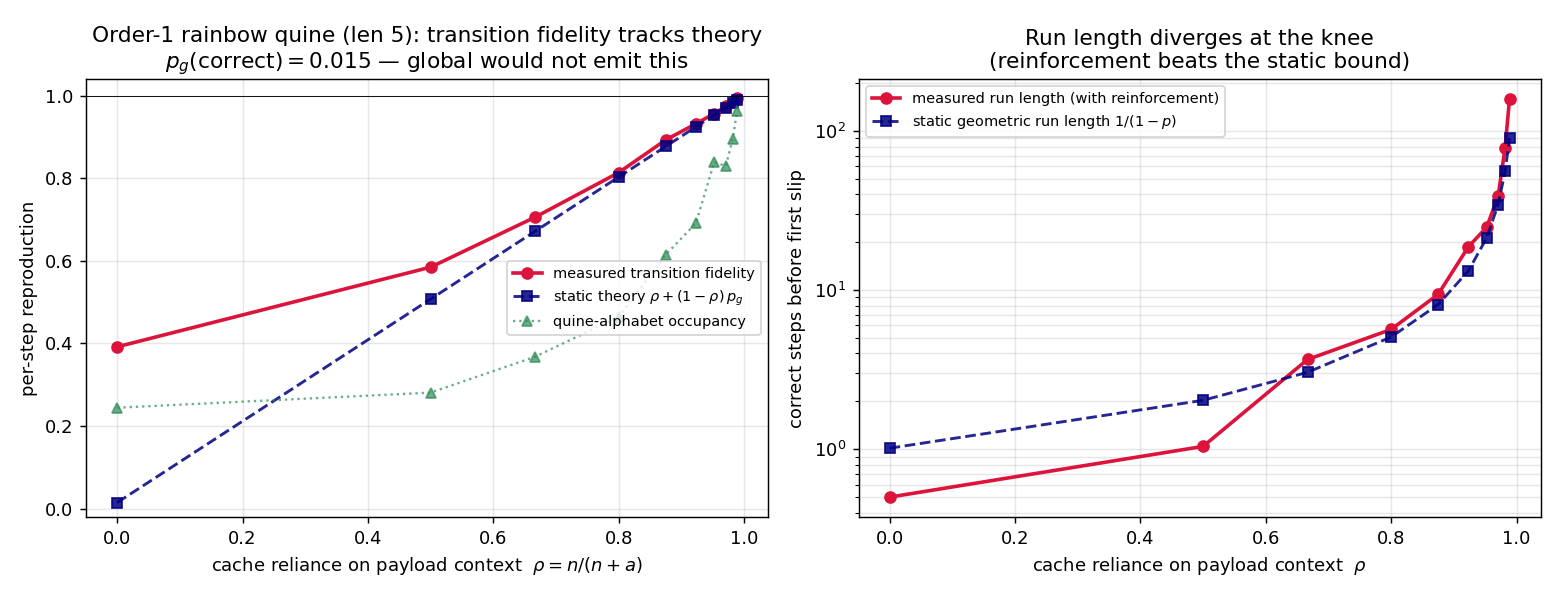
\includegraphics[width=\textwidth]{contagion_fidelity.png}
\caption{Order-$1$ rainbow quine over the rarest symbols ($\pg=0.015$). \emph{Left:} measured
transition fidelity tracks the closed form \eqref{eq:pstep}; alphabet occupancy lags but
$\to0.96$ (the walk re-enters after a slip). \emph{Right:} measured run length beats the
static geometric bound $1/(1-p_{\text{step}})$ once past the knee---self-reinforcement.
Reproduced by \texttt{demo\_contagion.py}.}
\label{fig:fidelity}
\end{figure}

\subsection{The order ladder and a window-distinctness theorem}\label{sec:orders}
The canonical exact quine at order $k$ is a de Bruijn cycle $B(2,k)$~\cite{debruijn1946} of
period $2^{k}$ over a two-symbol alphabet. Sweeping orders $2$--$5$ (Figure~\ref{fig:orders}) gives two facts. First,
\emph{per-step contagion is order-blind}: in the contagious regime every order tracks the same
\eqref{eq:pstep}. Second, \emph{brittleness is doubly exponential in order}: surviving one whole
period needs $p_{\text{step}}^{\,2^{k}}$, so the reproduced periods before a slip fall sharply
with $k$ (at $\rho=0.996$: $63,30,15,9$ periods for $k=2,\dots,5$). Order is a brittleness
dial, not a per-step one.

The following structural fact makes the divisibility question of \S\ref{sec:divis} well-posed.

\begin{theorem}[Window distinctness]\label{thm:window}
A cyclic string is an exact order-$k$ quine of genuine period $p$ if and only if its $p$
length-$k$ windows are all distinct. Consequently its de Bruijn subgraph is a single $p$-cycle
of out-degree-one nodes, which has no proper sub-cycle.
\end{theorem}
\begin{proof}
Exactness means each window has a single successor, i.e.\ each node of the order-$k$ de Bruijn
graph visited by $S$ has out-degree one; the walk $S$ is then a closed deterministic walk. If
some window recurred, determinism would force identical continuations from both occurrences,
making $S$ periodic with a proper divisor period---contradicting genuine period $p$. Hence the
$p$ windows are distinct and $S$ traces a simple $p$-cycle, which (all out-degrees being one)
contains no shorter closed walk. The converse is immediate. \end{proof}

We verified Theorem~\ref{thm:window} on $2157$ random exact quines (orders $1$--$4$, periods
$2$--$12$, alphabets $2$--$4$) with zero counterexamples. Its corollary is decisive: \emph{for
exact quines, period factorization is irrelevant}---there is no divisor sub-cycle to collapse
into. When the generated stream settles after a slip, it returns to the full period, never to a
proper divisor (confirmed across orders $2$--$5$). Divisibility can matter only once exactness
is relaxed.

\begin{figure}[t]
\centering
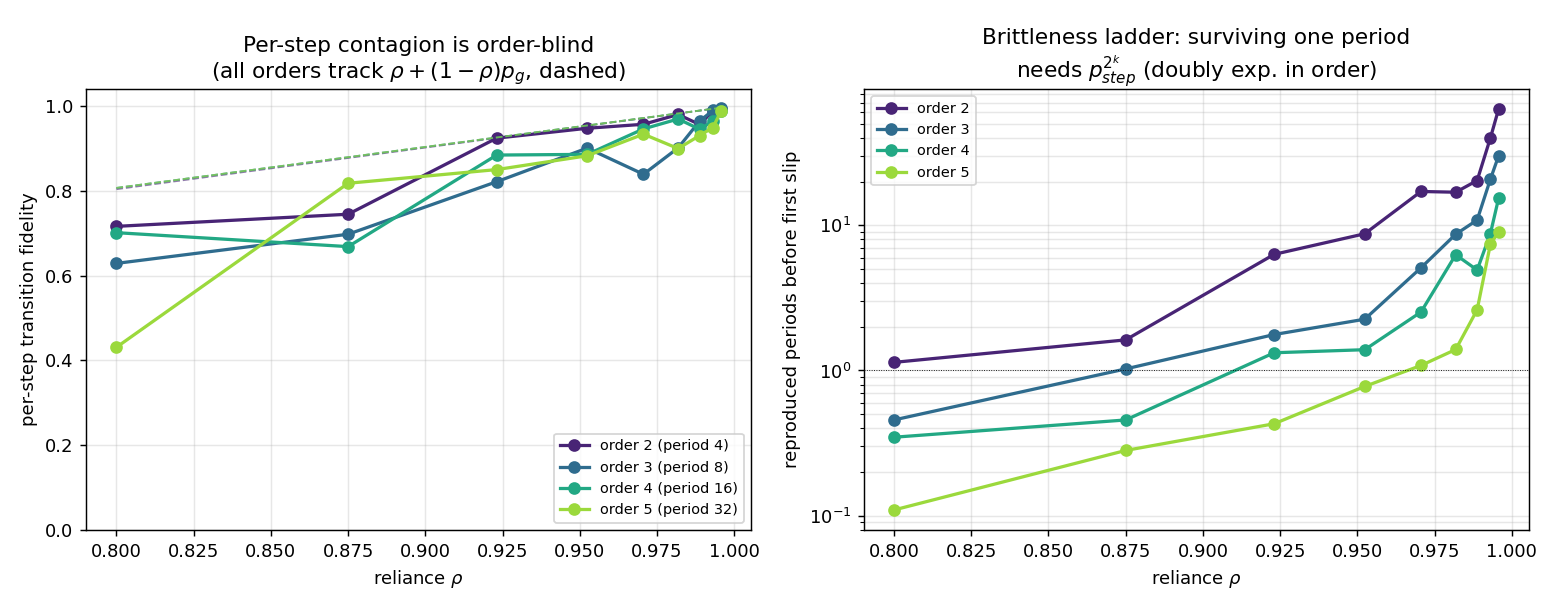
\includegraphics[width=\textwidth]{contagion_orders.png}
\caption{Order ladder, binary de Bruijn quines $B(2,k)$, $k=2$--$5$. \emph{Left:} per-step
fidelity is order-blind (all track \eqref{eq:pstep}). \emph{Right:} surviving one period needs
$p_{\text{step}}^{\,2^{k}}$, so reproduced periods fall steeply with order---the brittleness
ladder. Reproduced by \texttt{demo\_contagion\_orders.py}.}
\label{fig:orders}
\end{figure}

\subsection{Approximate quines: divisibility gates collapse}\label{sec:divis}
Relax exactness with a \emph{quasi-periodic} payload: $m$ blocks that share a period-$d$ motif
and differ only by a leading tag symbol, so the genuine period is $p=md$ but the order-$1$
structure is just the motif. Resolving the $m$ blocks (hence the full period) needs cache order
$\ge d$, because the disambiguating tag sits $d$ positions back; below that order the payload
collapses onto the period-$d$ sub-cycle, a divisor of $p$.

Taking $d$ to be $p$'s largest proper divisor and running an order-$1$ cache
(Figure~\ref{fig:divis}) confirms a sharp number-theoretic prediction: composite-period payloads
settle onto their largest proper divisor ($8\!\to\!4$, $9\!\to\!3$, $12\!\to\!6$, $15\!\to\!5$,
$16\!\to\!8$, $25\!\to\!5$), while \emph{prime}-period payloads ($7,11,13$) have no nontrivial
sub-motif and reproduce the full period. A prime period is \emph{harmonic protection}: the
string either reproduces or breaks to noise, but cannot phase-lock to a shorter cycle. Sweeping
cache order at fixed composite $p$, the divisor-collapse fraction falls to zero exactly at
$k=d$, the resolving order; but escaping the harmonic by raising order is not free---it is paid
in the brittleness of \S\ref{sec:orders}, so full reproduction needs jointly $k\ge d$ and high
reliance.

\begin{figure}[t]
\centering
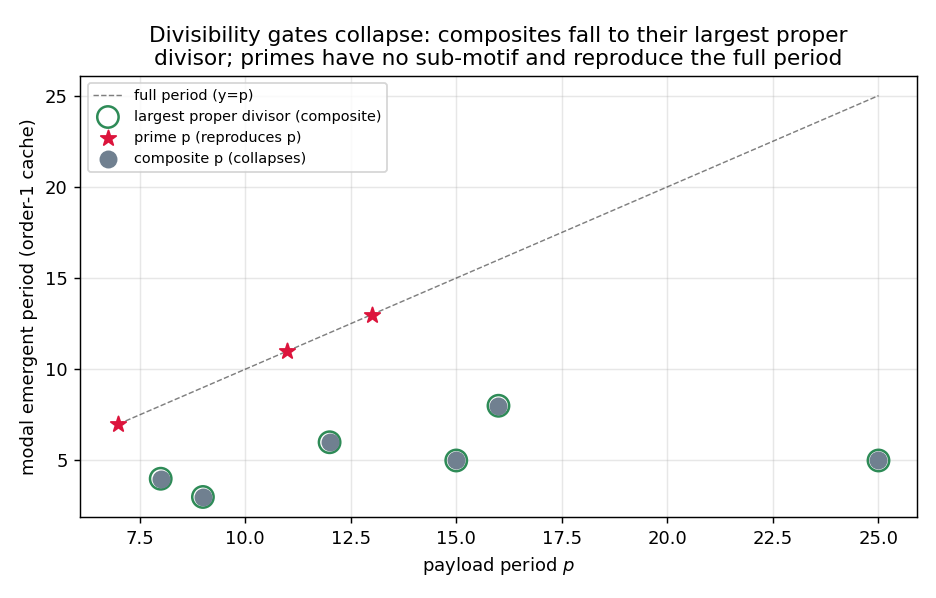
\includegraphics[width=0.72\textwidth]{contagion_divis_sweep.png}
\caption{Approximate (quasi-periodic) quines, order-$1$ cache. Composite periods collapse onto
their largest proper divisor (open circles); prime periods reproduce the full period (stars).
Divisibility gates the available sub-cycle attractors. Reproduced by
\texttt{demo\_contagion\_divis.py}.}
\label{fig:divis}
\end{figure}

\subsection{The cost of a payload: white-box versus black-box}\label{sec:regimes}
How much injection plants a quine to a target per-step probability $q$ (equivalently expected
run length $T=1/(1-q)$)? Because \eqref{eq:pstep} is exact, the answer is closed-form when the
global is known.

\begin{proposition}[Minimal payload]\label{prop:minreps}
For a self-loop payload with global prior $\pg$ on its transition, the minimal repetitions to
reach per-step probability $q$ under \eqref{eq:dir} is
\begin{equation}\label{eq:rstar}
\reps^{*}\;=\;a\,\frac{q-\pg}{1-q}\;=\;a\bigl(T(1-\pg)-1\bigr).
\end{equation}
\end{proposition}
\begin{proof}
Set $p_{\text{step}}=(\reps+a\pg)/(\reps+a)\ge q$ and solve for $\reps$. \end{proof}

A \emph{white-box} attacker who knows $\pg$ and $a$ simply evaluates \eqref{eq:rstar}. A
\emph{black-box} attacker, with only sampled generations, has a model-agnostic fallback: the
worst case $\pg=0$ gives $\reps_0=a(T-1)$, which \emph{guarantees} the target against any global
because reliance dominates the prior. The value of knowing the model is therefore the gap
\begin{equation}\label{eq:gap}
\reps_0-\reps^{*}\;=\;a\,T\,\pg,
\end{equation}
and it \emph{vanishes as $\pg\to0$}: against a maximally stealthy (rare) payload, knowing the
model buys the attacker nothing (Figure~\ref{fig:regimes}, left). With queries, an adaptive
doubling-plus-bisection search on a chosen-prefix one-step oracle recovers $\reps^{*}$, the
error shrinking as the inverse square root of queries spent (Figure~\ref{fig:regimes}, right).
Thus contagion is always achievable black-box, and black-box $\approx$ white-box exactly in the
adversarial corner.

\begin{figure}[t]
\centering
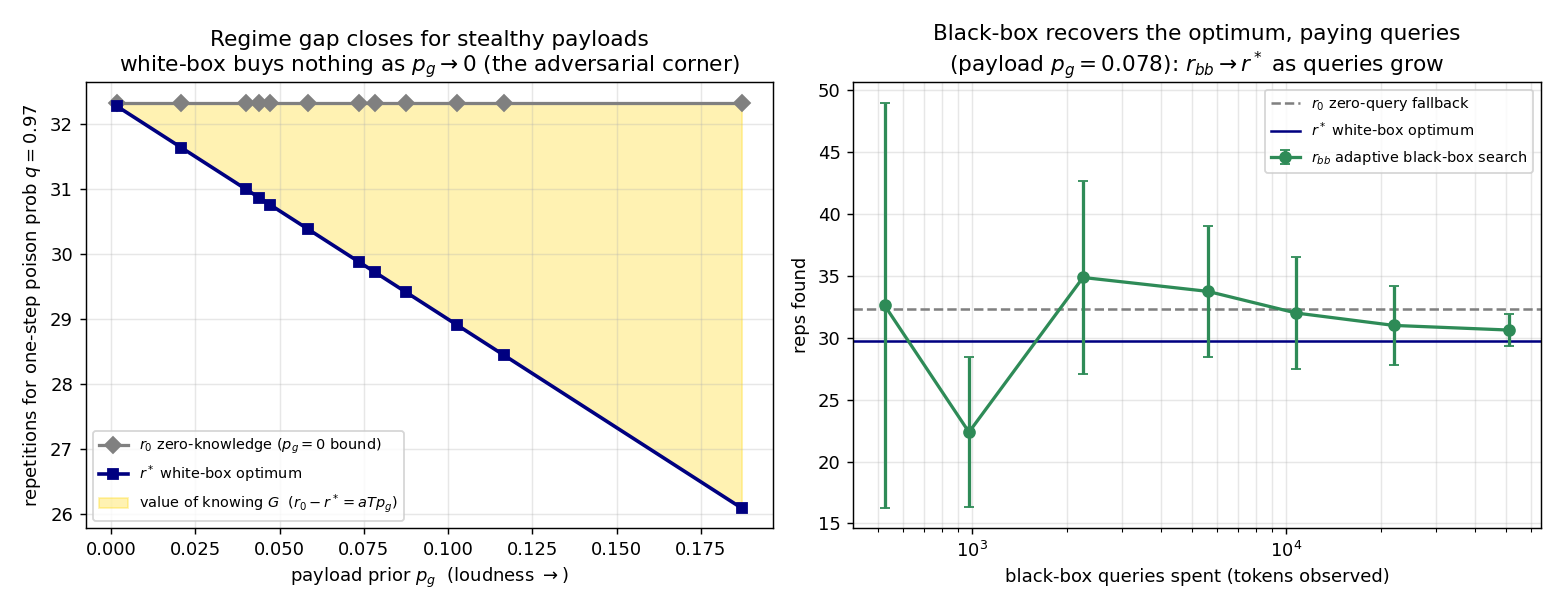
\includegraphics[width=\textwidth]{contagion_regimes.png}
\caption{Planting cost by attacker knowledge. \emph{Left:} the white-box optimum $\reps^{*}$ and
the zero-knowledge bound $\reps_0$; their gap $a\,T\,\pg$ (shaded) closes as the payload becomes
stealthier. \emph{Right:} an adaptive black-box search converges to $\reps^{*}$ as it spends
queries. Reproduced by \texttt{demo\_contagion\_regimes.py}.}
\label{fig:regimes}
\end{figure}

% ===========================================================================
\section{The delivery: infecting a trained cache}\label{sec:delivery}
% ===========================================================================
A realistic target is not an empty cache but one already \emph{warmed} on a legitimate document
$D$, whose generation rides $D$'s local structure. We take the payload token $\xstar$ to be
\emph{out-of-distribution}---a trigger the legitimate system never emits, sanitized out of the
corpus and $D$---so its contexts are fresh and its spontaneous emission rate is zero. The hijack
factors into two independent events:
\[
P(\text{hijack})\;=\;\underbrace{P(\text{enter the payload basin within }T)}_{\text{entry}}
\times
\underbrace{P(\text{lock-in}\mid\text{entered})}_{\text{condensation}} .
\]
Lock-in is the condensation of~\cite{shumow2026trust}; the new object is \emph{entry}.

\subsection{Entry, the bridge, and a frequency ceiling}\label{sec:entry}
To enter, generation must visit a context $c$ from which a poisoned transition routes to
$\xstar$. The attacker injects a \emph{bridge} edge $c\to\xstar$ with $w$ counts; the added
per-step entry rate is
\begin{equation}\label{eq:entryrate}
\text{freq}(c)\cdot P(\xstar\mid c)\;=\;\text{freq}(c)\cdot\frac{w}{n_c+w+a},
\end{equation}
the product of how often generation visits $c$ and the single-count leverage there. The two
factors trade off: frequent contexts are heavily warmed (high $n_c$, low leverage), so the best
\emph{bridge} is one both on $D$'s trajectory and under-warmed by this particular $D$
(Figure~\ref{fig:hijack}). Minimal poison to make entry likely ($P_{\text{enter}}\ge\frac12$
over a horizon of $T=60$ steps) is $3$ counts for the best bridge $\max\,\text{freq}(c)/(n_c+a)$, versus $8$ for the
most-visited context (penalized by its high $n_c$) and $13$ for a random one. A
\emph{frequency ceiling} bounds the whole approach: since $P(\xstar\mid c)\le1$, the entry rate
saturates at $\text{freq}(c)$, so a context with $\text{freq}(c)<-\ln(1-\text{target})/T$ can
\emph{never} reach the target however much poison is injected.

\begin{figure}[t]
\centering
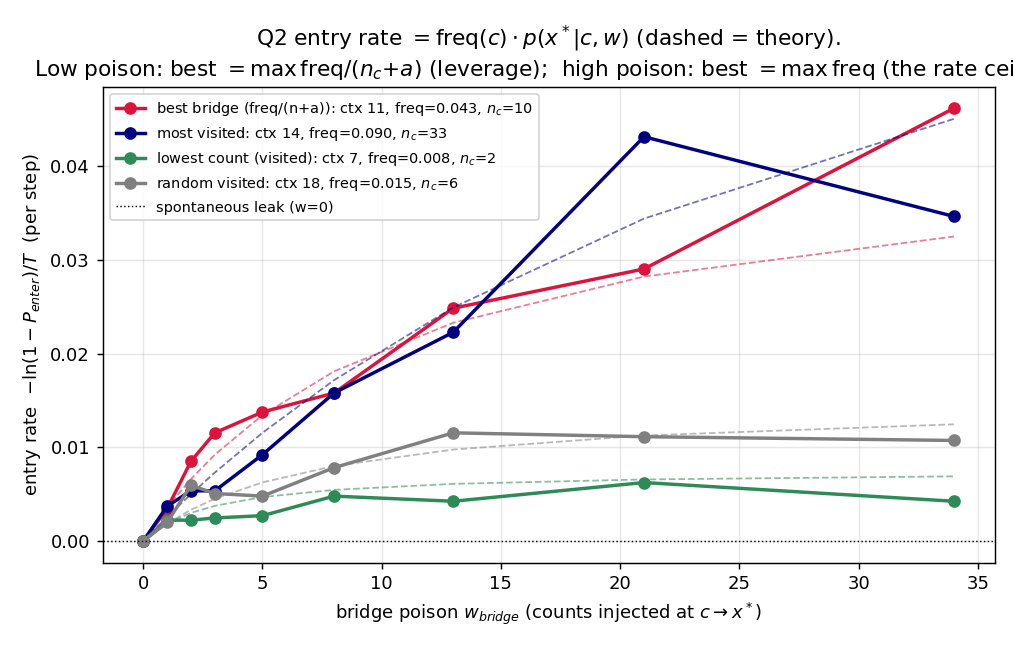
\includegraphics[width=0.78\textwidth]{contagion_hijack.png}
\caption{Entry into a cache warmed on $D$, payload $\xstar$ out-of-distribution (spontaneous
rate $0$ at $w=0$). A bridge adds entry rate \eqref{eq:entryrate} (dashed: theory). Low-poison
best bridge maximizes $\text{freq}/(n_c+a)$; high-poison entry rate $\to\text{freq}(c)$; low-frequency
contexts saturate below target (the ceiling). Reproduced by \texttt{demo\_contagion\_hijack.py}.}
\label{fig:hijack}
\end{figure}

\begin{remark}[Black-box entry-finding]\label{rem:bbentry}
The criterion that minimizes \emph{poison-to-target} is $\argmax_c(\text{freq}(c)-r)/(n_c+a)$
with $r$ the rate ceiling (not the marginal $\argmax_c\text{freq}(c)/(n_c+a)$; the two differ
near the ceiling). For this objective visit frequency dominates: a black-box attacker that only
\emph{watches} generations recovers the white-box-optimal bridge from observation alone
($\approx 2000$ tokens), and actively probing leverage is not worth its query cost. Defending the
entry surface therefore means watching for anomalous reliance on high-visit contexts---the
observable an attacker keys on.
\end{remark}

\subsection{Installing a contagious string, and the joint optimum}\label{sec:joint}
Bridging into a multi-symbol quine rather than a self-loop installs a contagious \emph{string}:
once entered, generation reproduces the cycle in order (measured tail cycle-fidelity
$0.79$--$0.97$ for lengths up to five), not merely visiting the payload alphabet. The total
poison then splits as a length-independent entry cost plus a payload cost $\reps\times p$ that
scales with string length.

Crucially, entry and lock-in are coupled---strong lock-in makes a single entry stick, so the
bridge can be cheap; weak lock-in demands an expensive bridge---so the cheapest hijack lives on
a two-dimensional frontier, not at either pinned extreme. Sweeping $(w,\reps)$ and reading the
minimal $w+\reps p$ on the $P(\text{hijack})\ge\frac12$ contour (Figure~\ref{fig:joint}), the
joint optimum sits at the condensation \emph{knee} ($\reps\!\in\![16,32]$), not at saturation,
and beats the ``pin lock-in strong'' recipe by $3$--$4\times$ (e.g.\ $48$ versus $136$ counts
at $p=1$; $192$ versus $648$ at $p=5$). Over-provisioning lock-in is wasted poison.

\begin{figure}[t]
\centering
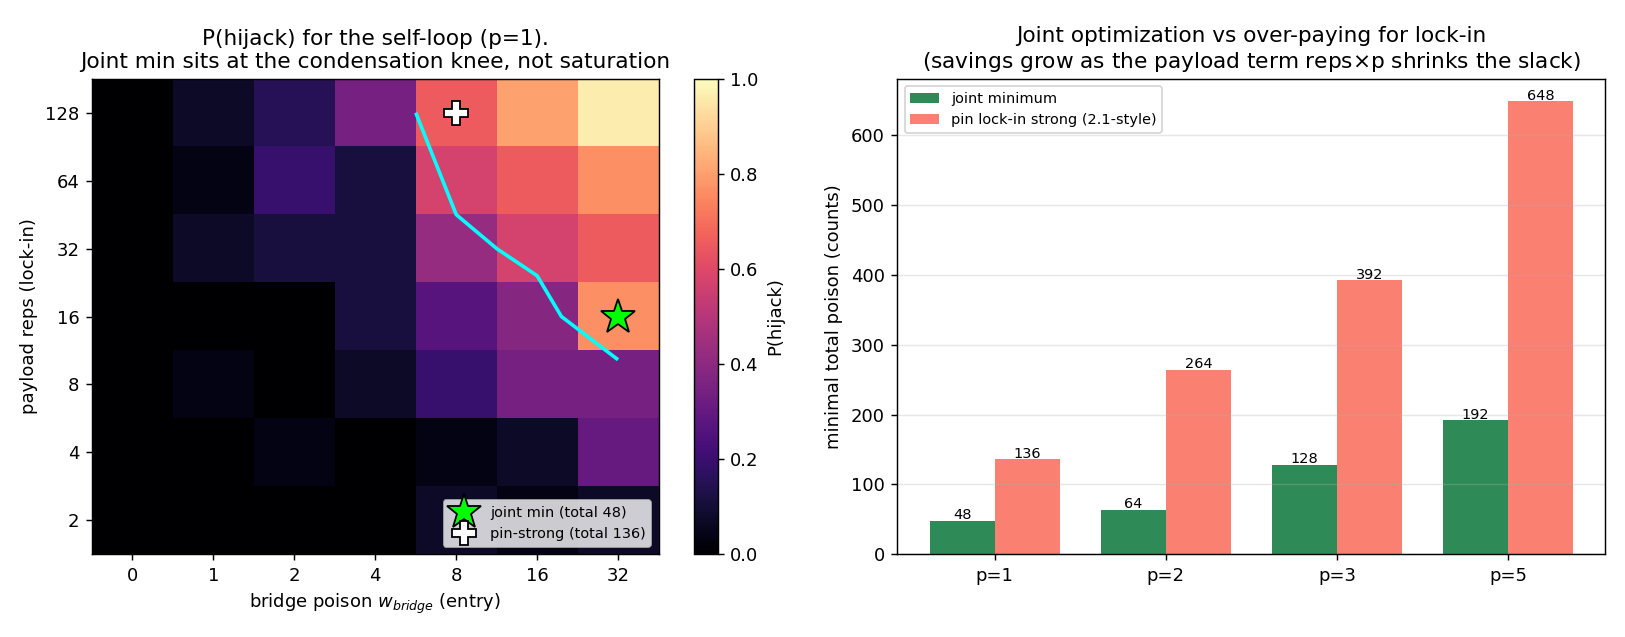
\includegraphics[width=\textwidth]{contagion_joint.png}
\caption{Joint minimal poison. \emph{Left:} $P(\text{hijack})$ over (entry $w$, lock-in $\reps$)
for a self-loop; the $\tfrac12$ contour (cyan) is L-shaped and the joint minimum (star) sits at
the knee, far below the pin-strong recipe (cross). \emph{Right:} joint minimum versus
over-provisioned lock-in across string lengths. Reproduced by \texttt{demo\_contagion\_joint.py}.}
\label{fig:joint}
\end{figure}

% ===========================================================================
\section{Transmission: a context-window worm}\label{sec:worm}
% ===========================================================================
Self-reproduction within one cache becomes \emph{contagion} when an infected output infects a
second host. The mechanism makes transmission a corollary of \S\ref{sec:payload}. An infected
host generates output in which the string $S$ appears $k$ times---its \emph{viral load}. A
second host that \emph{reads} that output streams those $k$ copies into its own cache, which is
exactly the payload injection of Proposition~\ref{prop:minreps} with $\reps=k$, and the read
context ends mid-string, so the receiver starts already inside the basin: \emph{secondary
infection needs no bridge}. The receiver then reproduces $S$ and re-broadcasts $k'$ copies in
its own $T$-token output. One passage is a map $k_{\text{in}}\mapsto k_{\text{out}}$, and the
epidemic is its iteration.

Two regimes follow (Figure~\ref{fig:worm}). Below a transmissibility threshold the receiver does
not reproduce and $k_{\text{out}}\approx0$ (the chain dies). Above it the receiver reproduces and
broadcasts a load $k_{\text{out}}\approx\text{(occupancy)}\cdot T/p$, a ceiling set by how much it
generates ($T$) divided by the string length ($p$). The basic reproduction
number~\cite{andersonmay1991} is the ratio of broadcast to threshold,
\begin{equation}\label{eq:R0}
\Rzero\;\approx\;\frac{\text{broadcast ceiling}}{\text{threshold}}\;\approx\;\frac{T}{p\,k_{\text{thresh}}},
\end{equation}
so contagiousness falls with string length and rises with how much each host emits. Serial
passage from a strong index host bears this out: a length-$1$ string climbs to an endemic load
($\sim\!90$ copies/host), length $2$ sustains near threshold, but lengths $\ge3$ die out within
a few passages. There is a \emph{critical string length} (here $\approx2$--$3$, scaling with
$T$) above which $\Rzero<1$ and the worm infects only the index host. Length trades payload
richness against transmissibility: the worm wants to be short.

\begin{figure}[t]
\centering
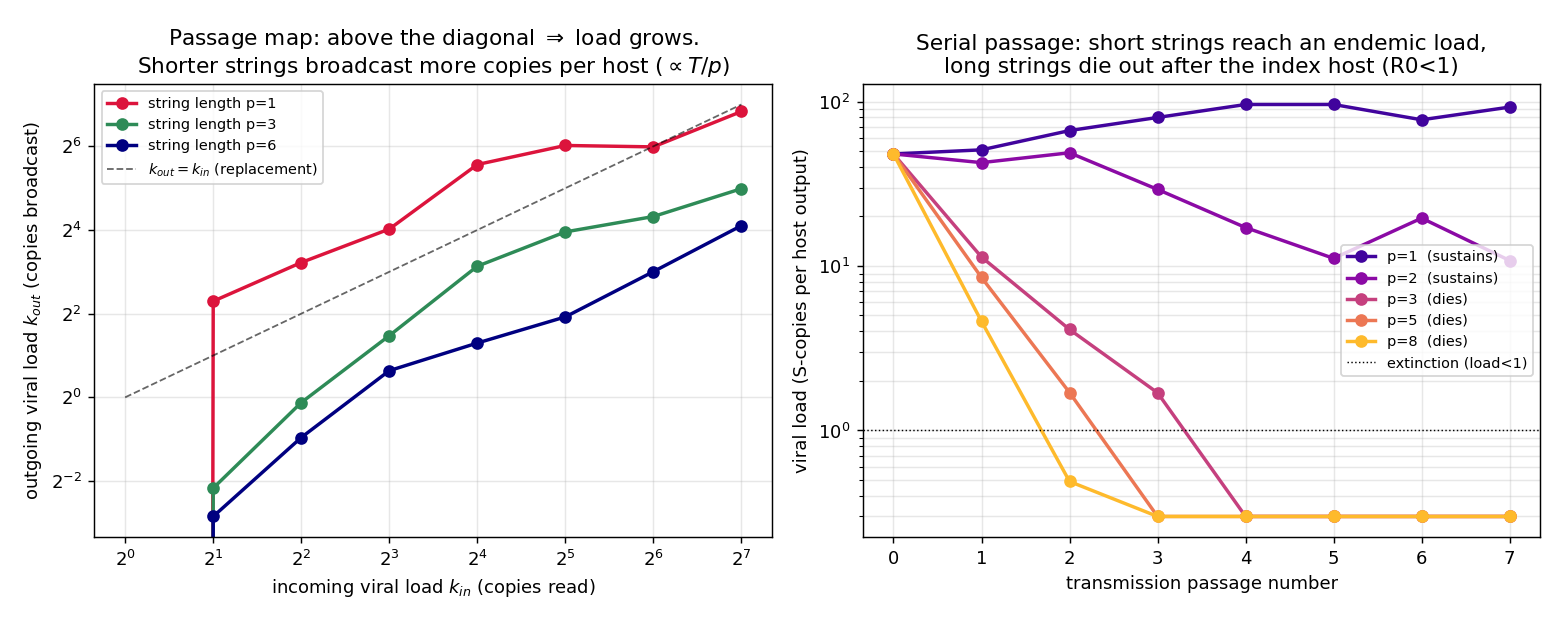
\includegraphics[width=\textwidth]{contagion_worm.png}
\caption{Cross-cache propagation. \emph{Left:} the passage map $k_{\text{in}}\!\to\!k_{\text{out}}$;
above the replacement diagonal the load grows ($p=1$, supercritical), below it the load decays
($p=3,6$). \emph{Right:} serial passage---short strings reach an endemic load, long strings die
out after the index host ($\Rzero<1$). Reproduced by \texttt{demo\_contagion\_worm.py}.}
\label{fig:worm}
\end{figure}

% ===========================================================================
\section{Under induction: the conjecture's mechanism in the toy}\label{sec:ppm}
% ===========================================================================
Everything so far used a fixed-order count cache, whose trust is the reliance $n/(n+a)$ of
\eqref{eq:reliance}---earned by accumulating counts. The conjecture (\S\ref{sec:discussion})
names a \emph{different} trust mechanism: induction, where a span is trusted because it
\emph{matches} a previous span, not because copying it helps. The toy ships exactly this as an
alternative cache. \texttt{PpmPredictor} is a variable-order online predictor that interpolates
the longest previously-seen suffix down to the global model with absolute discounting---``saw
$A\,B\dots$ now see $A$, predict $B$,'' an induction head built from counts~\cite{olsson2022}.
It is never told its order; it discovers the effective order per context. Swapping it in for the
count cache tests the conjecture's mechanism within the toy, where it stays exact.

The mechanistic contrast is sharp: the count cache needs many presentations to drive reliance
past the condensation knee, whereas induction earns near-full trust from a single long,
near-deterministic match. Three consequences follow
(Figures~\ref{fig:ppm},~\ref{fig:ppmworm}).

\paragraph{Cheaper to plant.} A rainbow quine reaches fidelity $0.9$ after about three
presentations under induction, versus $12$--$32$ for the count cache, and locks sharply to $1$
by the fourth (Figure~\ref{fig:ppm}, left). At a \emph{single} presentation induction is in
fact worse: a once-seen suffix keeps only $1-d$ of its mass under absolute discounting, so
induction must have seen a span at least twice before it copies it confidently---a small but
telling threshold.

\paragraph{Structural reach.} The brittleness ladder of \S\ref{sec:orders} is an artifact of
fixed order. For a de Bruijn $B(2,3)$, which needs order $3$, the order-$1$ cache cannot
reproduce it at all and an order-matched order-$3$ cache is brittle (fidelity $0.76$ at eight
presentations); induction reaches $0.9$ by the third presentation and $1$ by the sixth, never
told the order (Figure~\ref{fig:ppm}, right). It copies long-range structure a fixed low-order
count mechanism cannot represent.

\paragraph{More transmissible.} Re-running the worm of \S\ref{sec:worm} with induction hosts
collapses the transmissibility threshold. Because reproduction now needs only two or three
copies, $k_{\text{thresh}}$ in \eqref{eq:R0} falls accordingly and $\Rzero$ stays above one for
far longer strings: in serial passage every length we tried ($1$--$8$) sustains, each reaching
the full $T/p$ broadcast ceiling, where the count cache died for every length $p\ge3$
(Figure~\ref{fig:ppmworm}). The critical length jumps---long worms that count-trust kills are
viable under induction.

\begin{figure}[t]
\centering
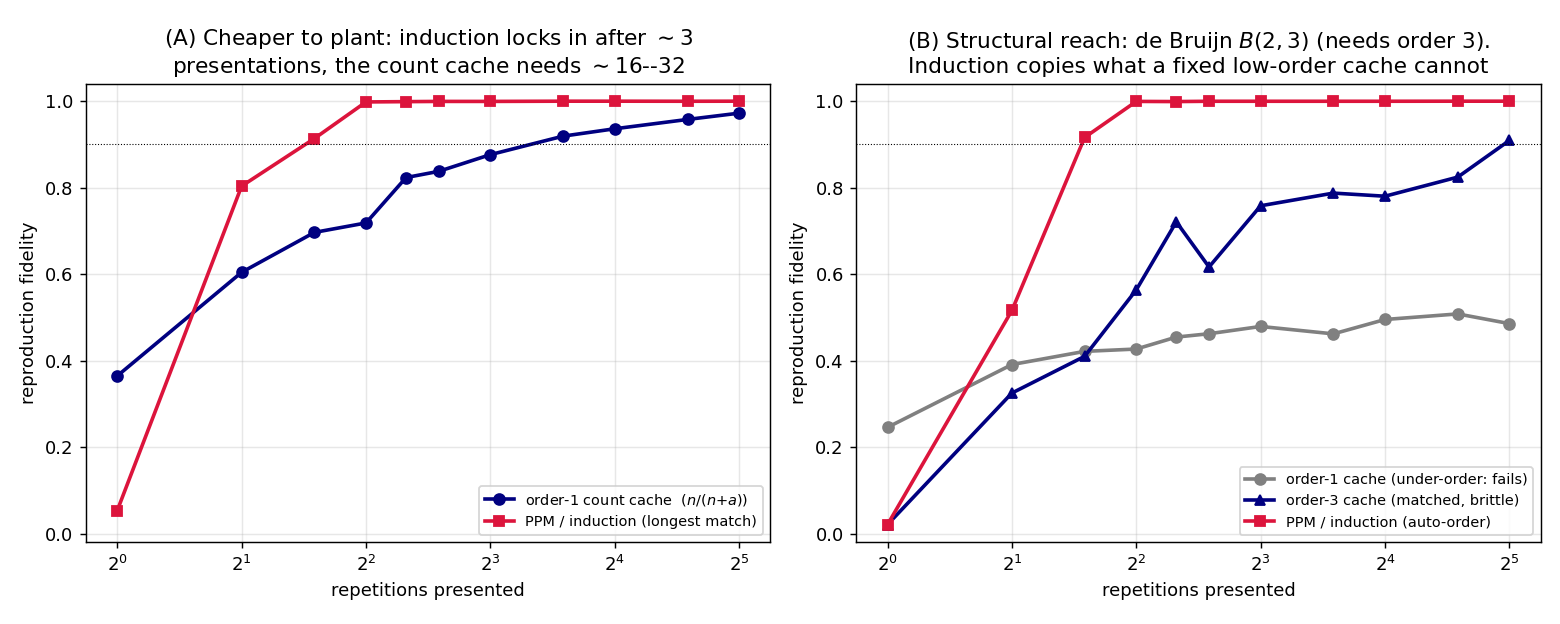
\includegraphics[width=\textwidth]{contagion_ppm.png}
\caption{Contagion under the induction surrogate (PPM) versus the fixed-order count cache.
\emph{Left:} a rainbow quine reproduces after $\sim3$ presentations under induction but $\sim16$--$32$
under counting. \emph{Right:} for a de Bruijn $B(2,3)$ (needs order $3$) the order-$1$ cache
fails and the order-$3$ cache is brittle, while induction---never told the order---reproduces it.
Reproduced by \texttt{demo\_contagion\_ppm.py}.}
\label{fig:ppm}
\end{figure}

\begin{figure}[t]
\centering
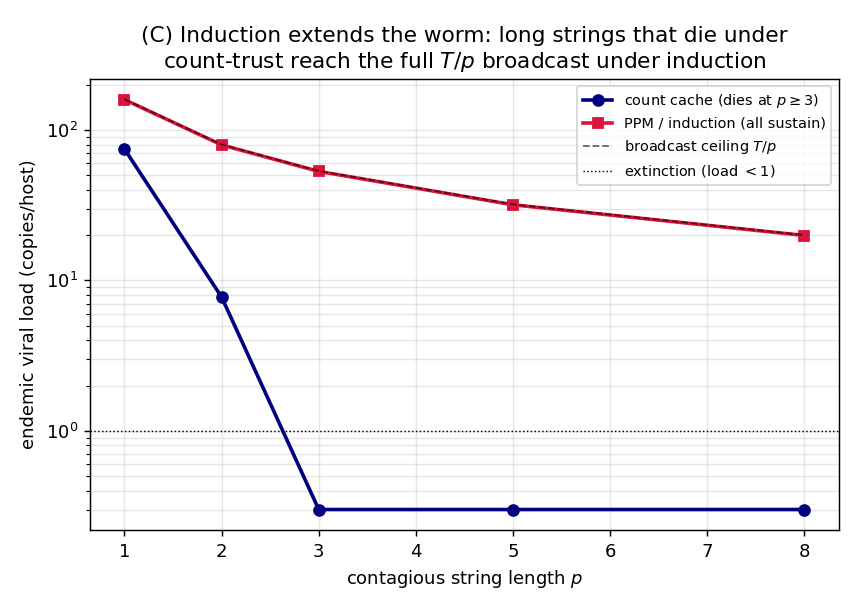
\includegraphics[width=0.62\textwidth]{contagion_ppm_worm.png}
\caption{The worm under induction. Serial-passage endemic load versus string length: the count
cache dies for $p\ge3$, but under induction every length sustains at the full $T/p$ broadcast
ceiling---the critical length jumps because $k_{\text{thresh}}$ collapses. Reproduced by
\texttt{demo\_contagion\_ppm.py}.}
\label{fig:ppmworm}
\end{figure}

The reading is that induction is not incidental to the conjecture but its engine: it is exactly
where self-reproducing strings are cheapest to plant, where the order and length penalties
vanish, and where transmission sustains longest. This is established on the toy, with the same
predictor the project uses as its induction surrogate. It does not by itself settle the
real-transformer question, but it removes the most obvious way the conjecture could have failed:
that the cheap, length-robust contagion seen above was a peculiarity of fixed-order
\emph{counting} rather than of trust-by-\emph{matching}.

% ===========================================================================
\section{Discussion}\label{sec:discussion}
% ===========================================================================
Three observations recur across the parts and are the load-bearing take-aways.

\paragraph{A single quantity threads the program.} Reliance \eqref{eq:reliance}---trust---sets
per-step fidelity \eqref{eq:pstep}, the lock-in probability, the payload cost \eqref{eq:rstar},
and the transmission threshold \eqref{eq:R0}. The condensation knee of~\cite{shumow2026trust} is
where strings begin to reproduce (\S\ref{sec:payload}), where the cheapest hijack sits
(\S\ref{sec:joint}), and where a worm becomes supercritical (\S\ref{sec:worm}). The paper is in
this sense a single statement about trust, told at three scales.

\paragraph{Black-box $\approx$ white-box where it matters.} Twice, independently, the
information an attacker lacks turns out not to help in the adversarial regime: knowing the global
model buys nothing against a stealthy payload \eqref{eq:gap}, and knowing the victim's warmed
counts buys nothing for entry-finding once visit frequency is observed
(Remark~\ref{rem:bbentry}). The practically dangerous attacks are the cheap, observation-only
ones.

\paragraph{Short and simple is contagious; long and rich is not.} Every length effect points the
same way. Higher-order, longer strings are doubly-exponentially more brittle to reproduce
(\S\ref{sec:orders}), cost $\propto p$ to plant (\S\ref{sec:joint}), and have $\Rzero\propto1/p$
to transmit (\S\ref{sec:worm}). A self-replicating context payload is under pressure to be a
short, low-order motif---which is also the regime a defender can most plausibly enumerate and
watch for.

\paragraph{Toward real transformers, and defenses.} As in~\cite{shumow2026trust} the bridge to
real models is a conjecture, but a sharper one here, and \S\ref{sec:ppm} has already supplied
its toy-level evidence. The induction (copy) mechanism~\cite{olsson2022} is precisely a
longest-match cache, so the de Bruijn determinism of \S\ref{sec:orders} and the
divisor-collapse of \S\ref{sec:divis} predict that highly templated or repetitive contexts---where
induction earns trust on grounds orthogonal to usefulness---are where short self-reproducing spans
are cheapest to plant and most transmissible, with prime-length (aperiodic) motifs the most
robustly self-locking. The defensive reading inverts the obvious instinct in a now-concrete way:
the quantity to bound is \emph{trust placed on high-visit, repetitive context}, and the cheapest
worms are short, so a watch-list of self-similar low-order spans, plus a cap on how much reliance
any recurring span can earn, attacks exactly the regime the cost analysis says an attacker will
use.

% ===========================================================================
\section{What is claimed, and what is not}\label{sec:honesty}
% ===========================================================================
Everything is established \emph{on the toy}, where the relevant objects are exact:
Theorem~\ref{thm:window} is a graph fact (and was checked computationally), \eqref{eq:pstep},
\eqref{eq:rstar}, \eqref{eq:gap}, \eqref{eq:entryrate} are algebra on \eqref{eq:dir}, and the
condensation and epidemic thresholds are standard reinforced-process and branching phenomena read
off a literal Markov chain. The constructed correspondences---``payload / delivery / worm'' and the
epidemiological $\Rzero$---are organizing devices, not theorems about transformers. The
induction results of \S\ref{sec:ppm} use the project's longest-match predictor (PPM); they show
the phenomena are a property of trust-by-matching rather than of fixed-order counting, but PPM
is a model of an induction head, not a transformer. The
divisibility result is exact for the quasi-periodic construction but should not be over-read: it
says period factorization gates \emph{which} sub-cycles exist, not that natural strings are
prime-protected. The joint-poison minima are grid-resolution upper bounds; the $3$--$4\times$
saving and the ``minimum at the knee'' structure are the robust claims. The transformer
conjecture of \S\ref{sec:discussion} is stated to be attacked, not assumed. What we do claim
firmly is the qualitative skeleton: self-reproducing context strings exist and are characterized
by window-distinctness and reliance; they can be planted in an occupied cache for a poison budget
that is cheapest at the condensation knee and is no harder black-box than white-box where it
matters; and their cross-host spread has a reproduction number that falls with length, with a
critical length above which contagion does not sustain.

\begin{thebibliography}{9}
\bibitem{shumow2026trust} D.\ Shumow. \emph{Trust Is the Attack Surface: A Cryptanalytic Reading
of In-Context Memory Poisoning in a Markov Mixture Model.} Companion write-up, project
\texttt{trust-is-the-attack-surface}, 2026.

\bibitem{cohen2024} S.\ Cohen, R.\ Bitton, B.\ Nassi. \emph{Here Comes the AI Worm: Unleashing
Zero-click Worms that Target GenAI-Powered Applications.} 2024.

\bibitem{greshake2023} K.\ Greshake, S.\ Abdelnabi, S.\ Mishra, C.\ Endres, T.\ Holz,
M.\ Fritz. \emph{Not What You've Signed Up For: Compromising Real-World LLM-Integrated
Applications with Indirect Prompt Injection.} AISec, 2023.

\bibitem{bietti2023} A.\ Bietti, V.\ Cabannes, D.\ Bouchacourt, H.\ J\'egou, L.\ Bottou.
\emph{Birth of a Transformer: A Memory Viewpoint.} NeurIPS, 2023.

\bibitem{olsson2022} C.\ Olsson et al. \emph{In-context Learning and Induction Heads.}
Transformer Circuits, 2022.

\bibitem{debruijn1946} N.\ G.\ de Bruijn. \emph{A Combinatorial Problem.} Proc.\ Koninklijke
Nederlandse Akademie van Wetenschappen, 1946.

\bibitem{pemantle2007} R.\ Pemantle. \emph{A Survey of Random Processes with Reinforcement.}
Probability Surveys, 2007.

\bibitem{andersonmay1991} R.\ M.\ Anderson, R.\ M.\ May. \emph{Infectious Diseases of Humans:
Dynamics and Control.} Oxford University Press, 1991.
\end{thebibliography}

\end{document}
